\newpage
\section{Parametrized Neural Network}
\subsection{Discriminating Masses}
When introducing the \ac{PNN} in section \ref{subsec:PNN}, I mentioned that by including the masses of the introduced particles as features 
in the feature set, we motivate individual tuning for each mass combination in the signal set. To study this, I will in this section 
present results where I manually assign all the events, both background and signal, the same parameters (mass combinations) thereby assigning 
most of the signal the wrong parameters. The hope is that if indeed the \ac{PNN} has been able to tune individually for each mass combination, 
then the \ac{PNN} should perform best when each signal event is given the correct parameter in the feature set. In other words, when each signal 
event is given the mass of the chargino and neutralino which was used when generating that specific event.
\\
In figure \ref{fig:PNN50250Dist} I have drawn the distribution of the output from the trained \ac{PNN} architecture 
(see section \ref{subsec:PNNArch}). The model was trained using the complete signal grid. In figure \ref{fig:PNN50250Dist},
4 signals have been included; $\{50,250\}_{GeV}$, $\{100,200\}_{GeV}$, $\{200,300\}_{GeV}$, and $\{150,250\}_{GeV}$. All data, including 
both signal and background were given the parameters of $50$ and $250$ (corresponding to the masses $\{50,250\}_{GeV}$) in the feature set. 
In figure \ref{fig:PNN50250Dist} the full output range is included, whereas in figure \ref{fig:PNN50250Dist_95} a cut off $0.975$ is placed on the 
output and therefore only includes the output in the range $[0.975-1]$. In both figures, it is evident that all mass combinations have been 
effectively separated from the background, even for the combinations which are given the wrong parameters (i.e. $\{100,200\}_{GeV}$, $\{200,300\}_{GeV}$, 
and $\{150,250\}_{GeV}$). Nevertheless, upon close study of figure \ref{fig:PNN50250Dist_95} and the corresponding legend, we can deduce that the signal 
which is given the correct parameters ($\{50,250\}_{GeV}$) is also the signal which is able to conserve the highest percentage of events when applying a 
simple cut off $0.975$\footnote{This is further evident when studying the efficiency percentages in table \ref{table:PNNSigComp}.}.\\
\begin{figure}
    \makebox[0.95\linewidth][c]{%
    \centering
    \begin{subfigure}{.5\textwidth}
        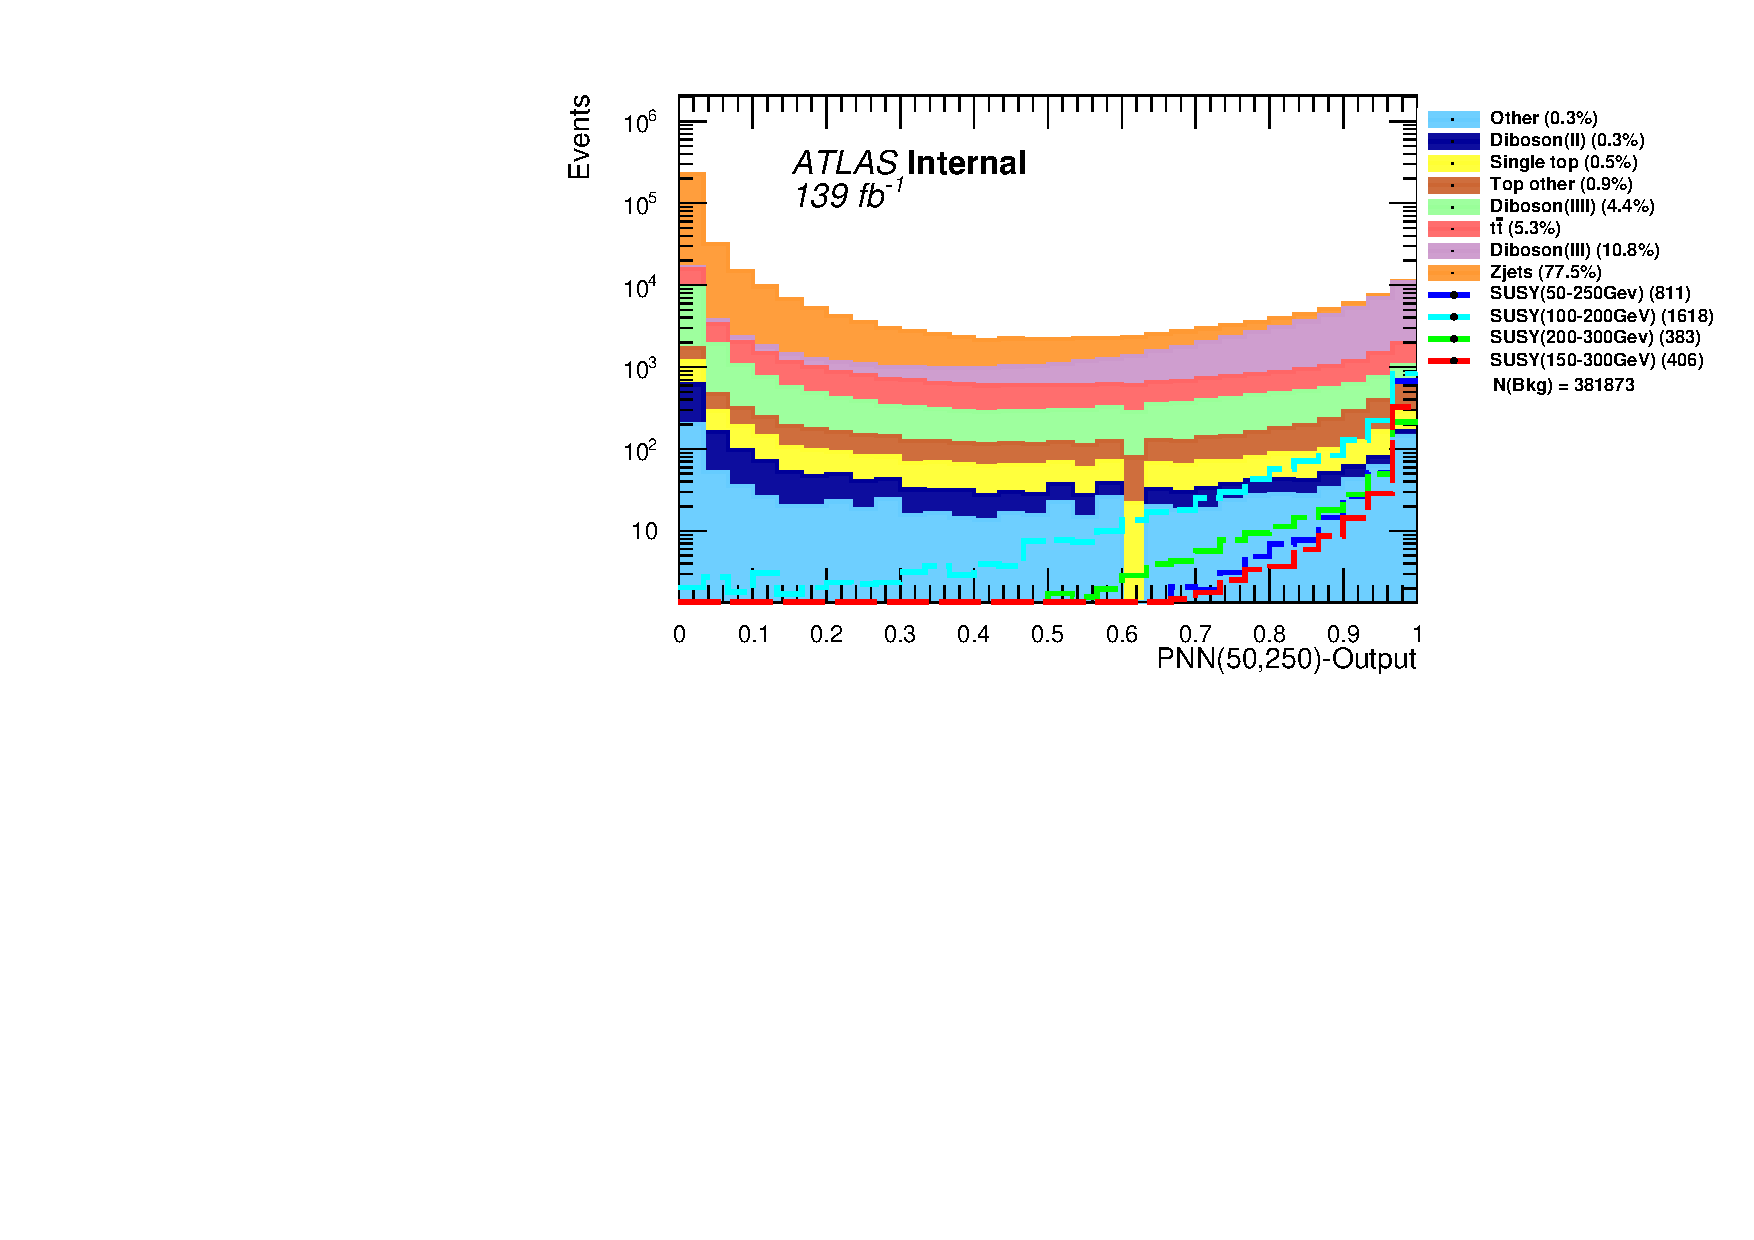
\includegraphics[width=\textwidth]{Figures/MLResults/NN/SUSY/MLDist/PNNDistTest/PNN50250Dist.pdf}
        \caption{}
        \label{fig:PNN50250Dist}
    \end{subfigure}
    \hspace{0cm}
    \begin{subfigure}{.5\textwidth}
        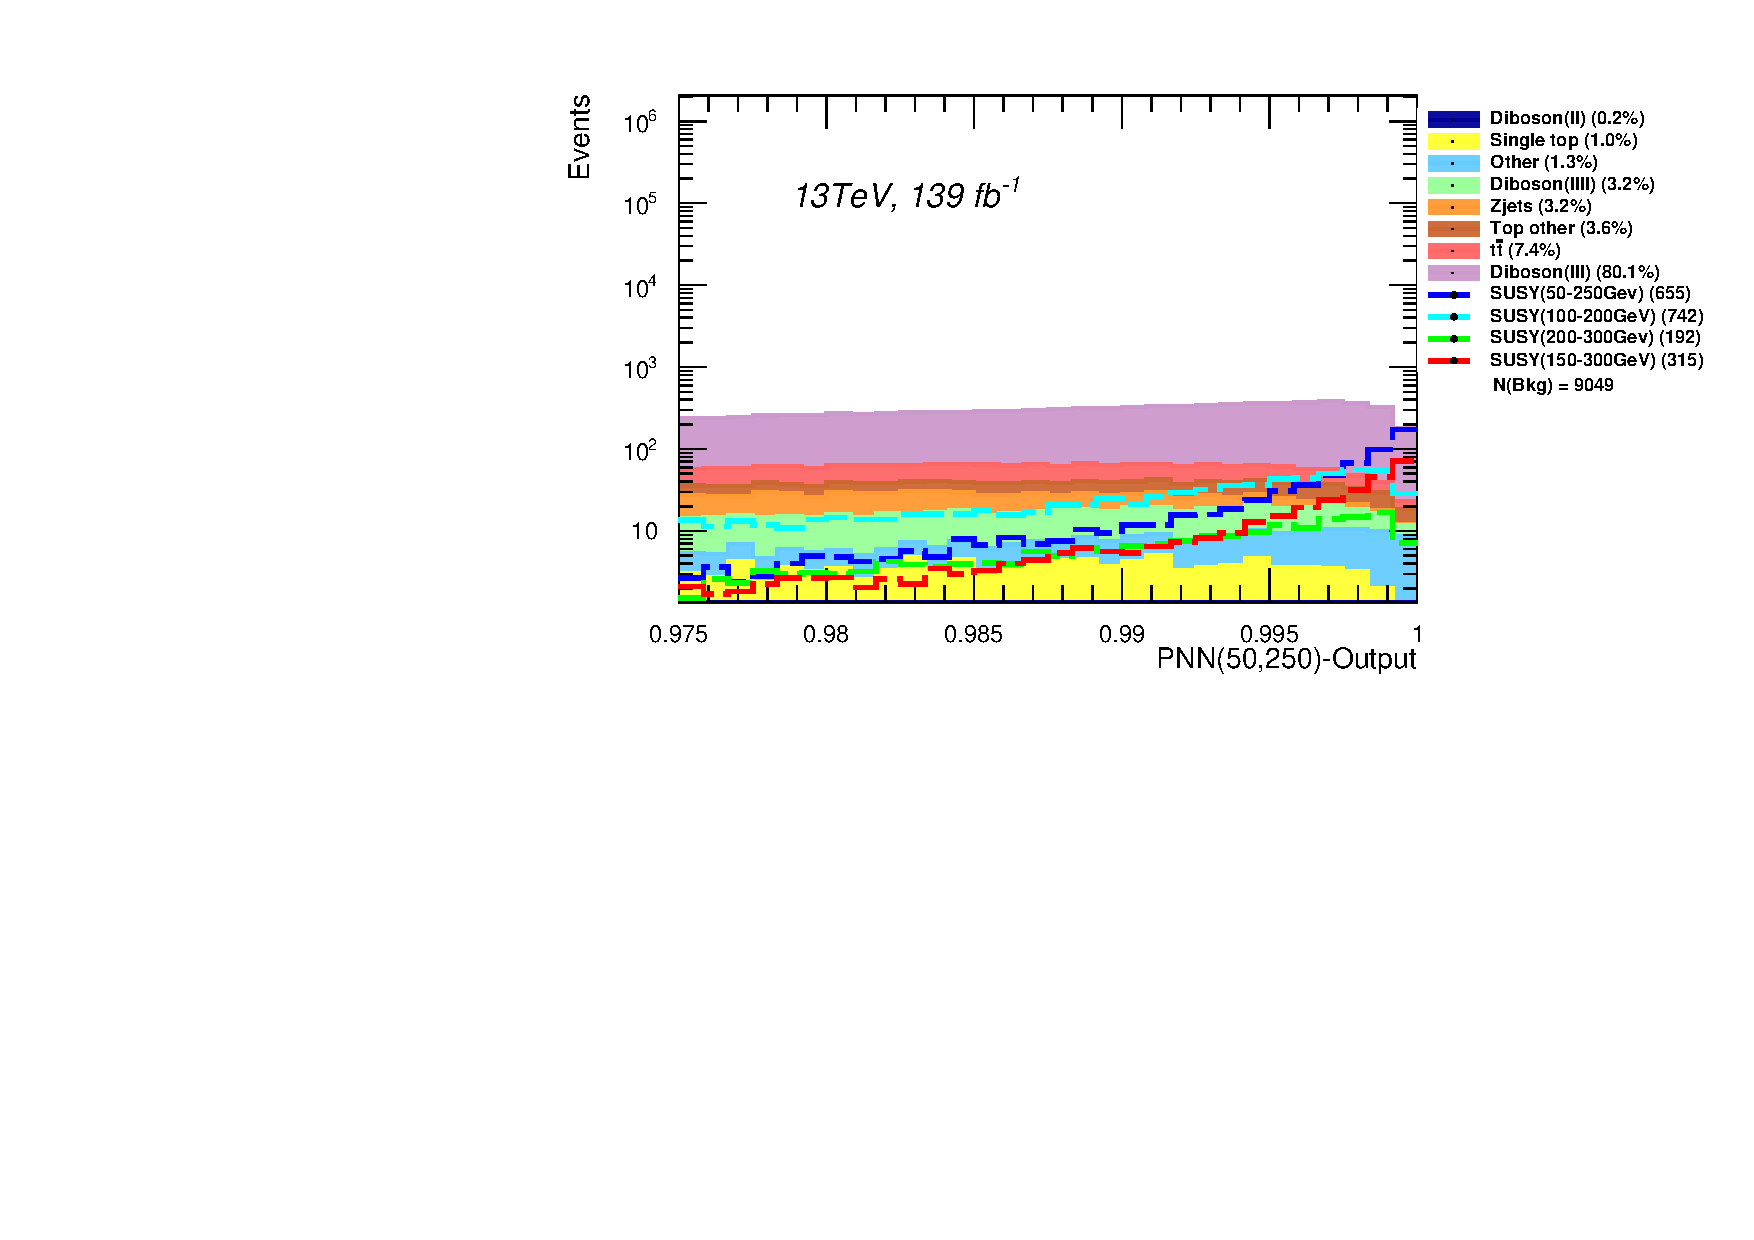
\includegraphics[width=\textwidth]{Figures/MLResults/NN/SUSY/MLDist/PNNDistTest/PNN50250Dist_C7.pdf}
        \caption{}
        \label{fig:PNN50250Dist_95}
    \end{subfigure}
    }
    \caption[The output distribution from a trained \acs{PNN} model for the background and signals with four different mass combinations, where 
    all events are given the same parameter.]{The output distribution from a trained \ac{PNN} model for the background and signals with four different 
    mass combinations: $\{50,250\}_{GeV}$, $\{100,200\}_{GeV}$, $\{200,300\}_{GeV}$, and $\{150,250\}_{GeV}$, and where all the data were given the 
    parameters corresponding to the masses $\{50,250\}_{GeV}$. The figure includes the full output range (\ref{fig:PNN50250Dist}) 
    and the output ranging from 0.975-1.00 (\ref{fig:PNN50250Dist_95}). The number in parentheses indicate the fraction of each background and 
    the absolute number of events for each signal point. The total number of background events is also shown.}
    \label{fig:PNN50250}
\end{figure} 
In section \ref{sec:XGBoost} I presented results indicating that some signals were easier to separate from background than others. This leads me to the 
question; did the \ac{PNN} perform better on the events with masses $\{50,250\}_{GeV}$ because it was given the correct parameters in the feature set, or simply
because this particular signal was easier to separate. To answer this question I conducted a second test. In figure \ref{fig:PNN200300DistComp} 
I repeated the analysis described in the paragraphs above, but where all the signals were given the parameter corresponding to the masses $\{200,300\}_{GeV}$.
Similarly to the previous results, I drew the output for the full output range (\ref{fig:PNN200300Dist}) and after a cutoff off $0.975$ (\ref{fig:PNN50250Dist_95}).
Via the examination of the two figures, we can indeed see that my assumption was right. Despite the fact that events with masses equal to  $\{50,250\}_{GeV}$
are given the wrong parameter, the \ac{PNN} still achieves the highest efficiency when predicting on the aforementioned events. \\
\begin{figure}
    \makebox[0.95\linewidth][c]{%
    \centering
    \begin{subfigure}{.5\textwidth}
        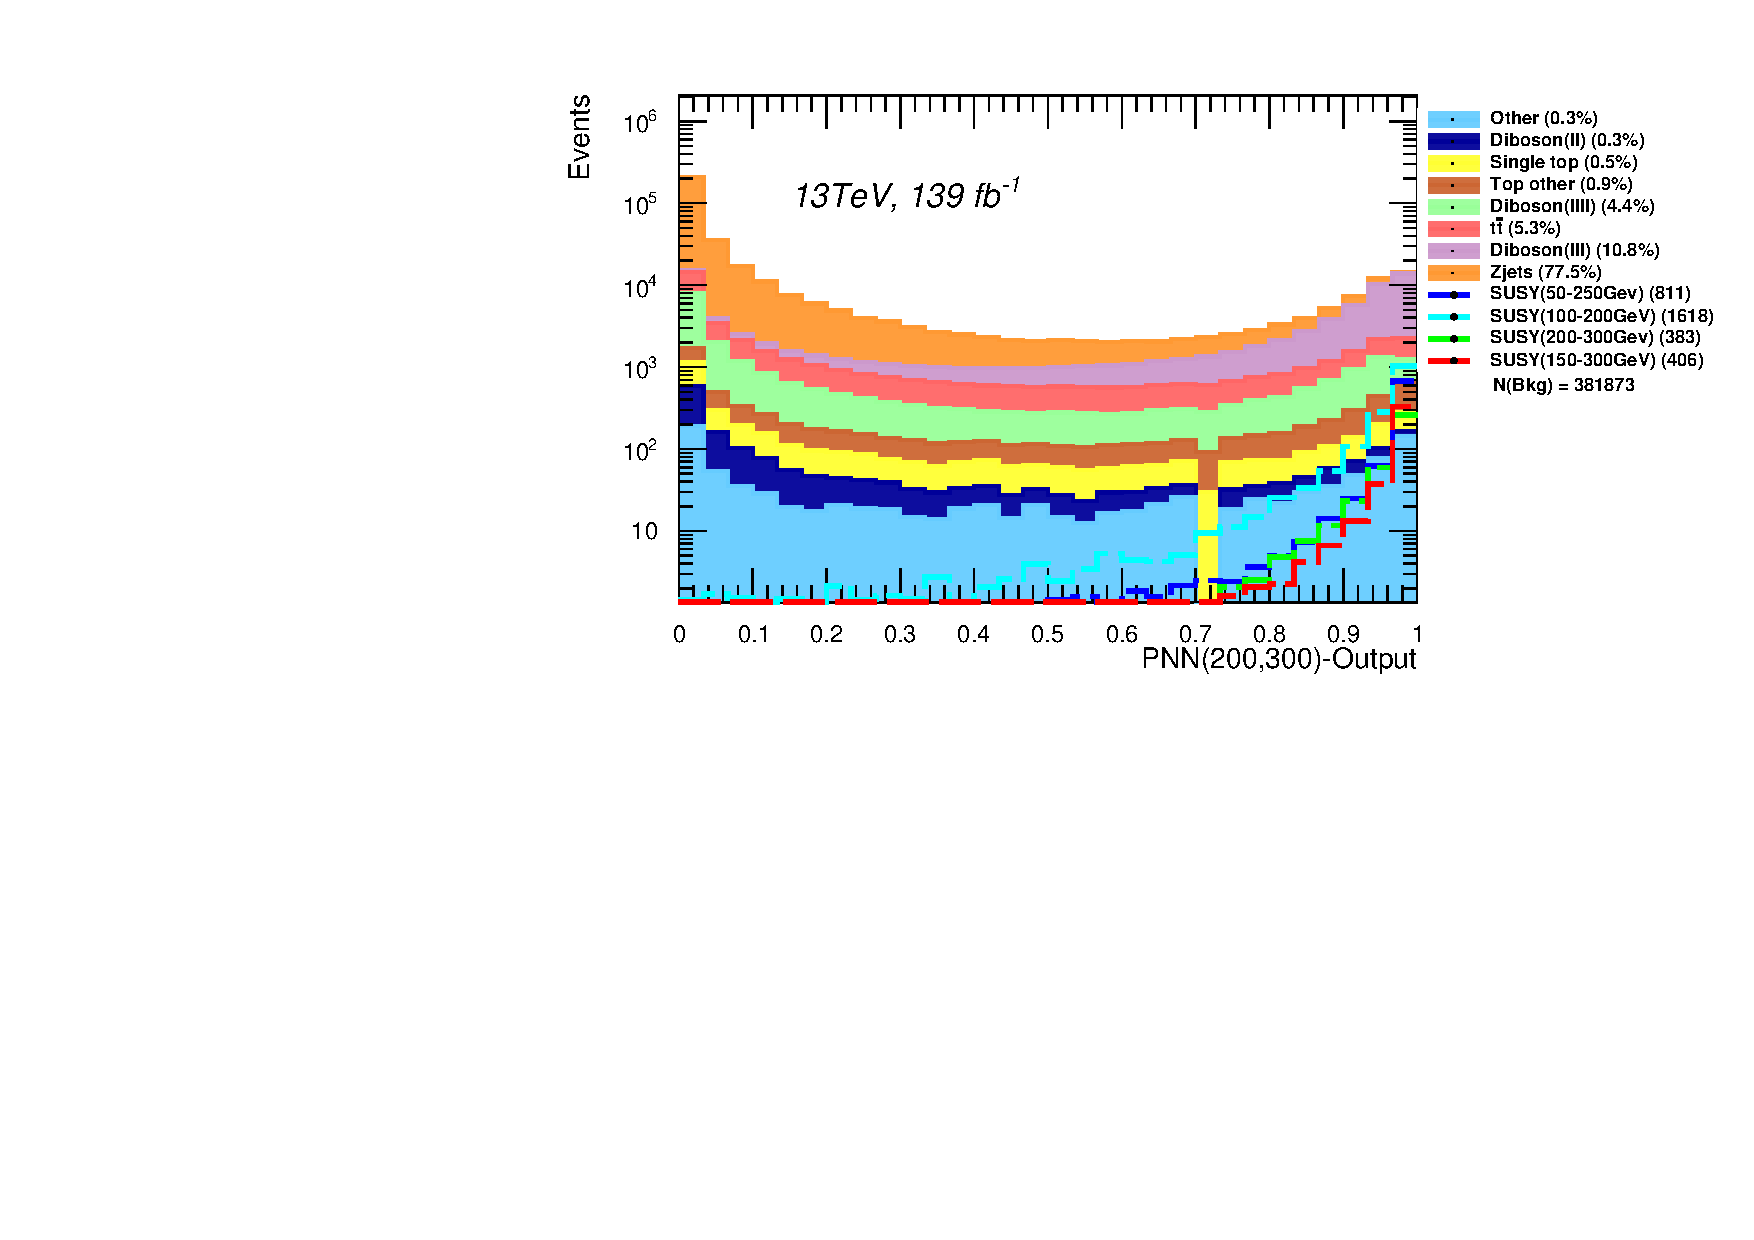
\includegraphics[width=\textwidth]{Figures/MLResults/NN/SUSY/MLDist/PNNDistTest/PNN200300Dist.pdf}
        \caption{}
        \label{fig:PNN200300Dist}
    \end{subfigure}
    \hfill
    \begin{subfigure}{.5\textwidth}
        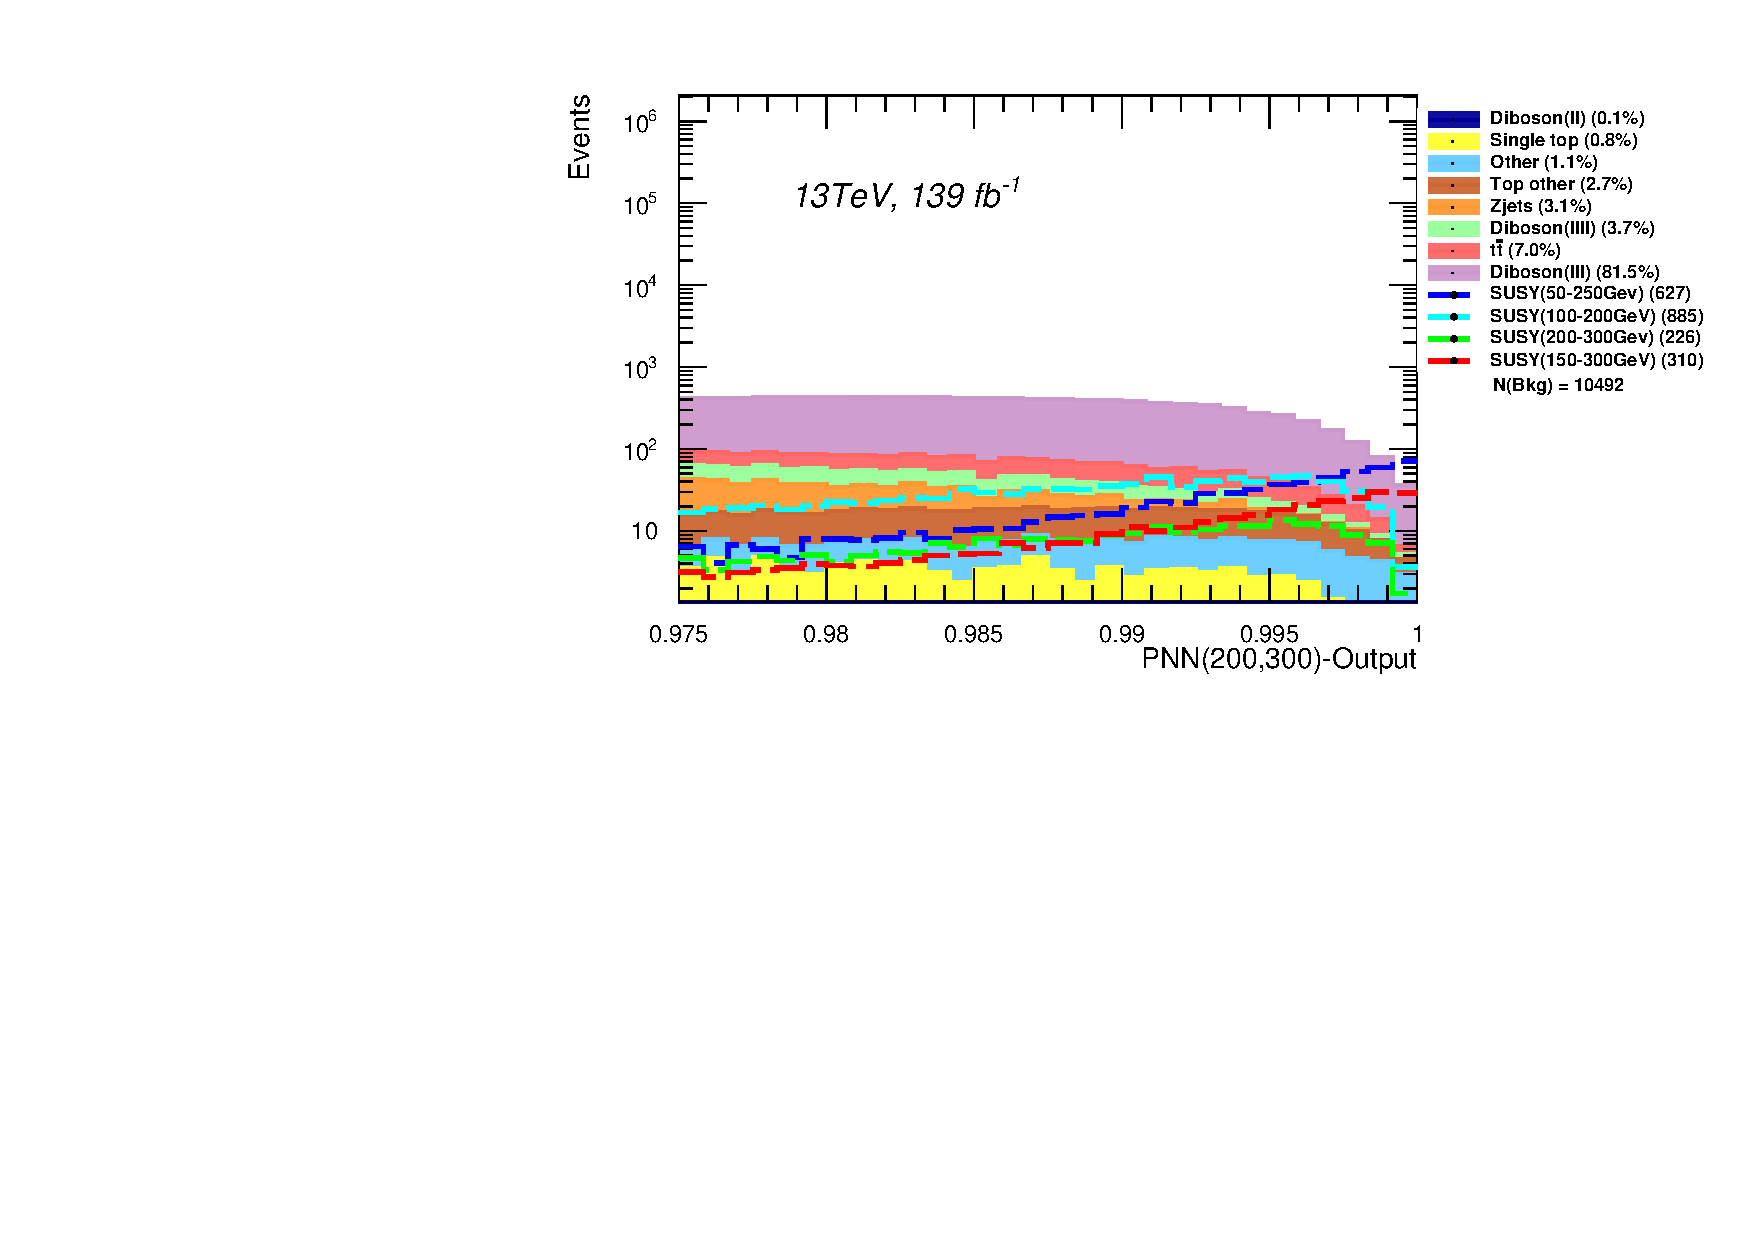
\includegraphics[width=\textwidth]{Figures/MLResults/NN/SUSY/MLDist/PNNDistTest/PNN200300Dist_C7.pdf}
        \caption{}
        \label{fig:PNN200300Dist_95}
    \end{subfigure}
    }
    \caption[The output distribution from a trained \acs{PNN} model for the background and signals with four different mass combinations, where 
    all events are given the same parameter.]{
    The output distribution from a trained \ac{PNN} model for the background and signals with four different mass combinations:
    $\{50,250\}_{GeV}$, $\{100,200\}_{GeV}$, $\{200,300\}_{GeV}$, and $\{150,250\}_{GeV}$, and where all the data were given the 
    parameters corresponding to the masses $\{200,300\}_{GeV}$. The figure includes the full output range (\ref{fig:PNN200300Dist}) 
    and the output ranging from 0.975-1.00 (\ref{fig:PNN200300Dist_95}). The number in parentheses indicate the fraction of each background and 
    the absolute number of events for each signal point. The total number of background events is also shown.}
    \label{fig:PNN200300DistComp}
\end{figure}
To further study this result, I created a table of the efficiencies of each mass combination for both results, after applying a simple cut of $0.975$. The results are presented in 
table \ref{table:PNNSigComp}. It is evident from table \ref{table:PNNSigComp} that the \ac{PNN} achieves the highest performance when events are given the correct label, 
although not by much. In the events with masses  $\{50,250\}_{GeV}$, the efficiency improved by a little over $3\%$, while the events with masses 
$\{200,300\}_{GeV}$, improved efficiency by almost $10\%$. Another interesting observation is that events with masses $\{100,200\}_{GeV}$ perform 
better when given the parameter of $\{200,300\}_{GeV}$ compared to $\{50,250\}_{GeV}$, despite the latter mass combination being closer in mass. 
A possible explanation is that the difference in mass ($\Delta m = |m_{\tilde{\chi}_1} - m_{\tilde{\chi}_2}|$), influences the feature distribution in the data, similarly 
to what we saw that size of mass does. Regardless, from \ref{table:PNNSigComp}, we can deduce that the \ac{PNN} does in fact discriminate between mass combinations 
and tune for them independently. 
\begin{table}[H]
    \centering
    $
    \begin{array}{ccccc}
        \hline \text { \backslashbox{\textbf{Parameters}}{\textbf{Channel}} }  & \text {$(50,250)$}& \text {$(100,200)$} & \text {$(150,300)$} & \text {$(200,300)$} \\
        \hline\text {$(50,250)$}   & \text { $\bf{80.8}\%$ } & \text { $45.8\%$ } & \text { $\bf{77.5}\%$ } & \text { $50.1\%$ } \\
        \hline\text {$(200,300)$}   & \text { $77.3\%$ } & \text { $\bf{54.6}\%$ } & \text { $76.3\%$ } & \text { $\bf{59.0}\%$ } \\
        \hline
    \end{array}
    $
    \caption{A listing of the remaining procentages of each mass combination after applying a cut of 0.975. The results are from a \ac{PNN} where all 
    of the events were given the parameters corresponding to the masses $\{50,250\}_{GeV}$ and $\{200,300\}_{GeV}$, respectively.}
    \label{table:PNNSigComp}
\end{table}

\subsection{Sensitivity Result}
In this section I will present the achieved sensitivity by the \ac{PNN} on the original signal set. In figure \ref{fig:PNNGridSig}, I present a grid displaying the sensitivity 
of the \ac{PNN} on the original signal set. Similarly to the previous models', the figure indicates that the \ac{PNN} is able to achieve a much higher sensitivity on the lower
masses. The most notable difference to the previous models, is the span of values for the significance. The \ac{PNN} almost doubles the highest significance achieved by any previous model
(from 2.44 to 4.14), and simultaneously achieves the lowest significance (now 0.30). The most probable explanation to this result is the distribution of parameters for the background. 
In section \ref{subsec:PNN}, I described how the background was randomly assigned the mass parameters using the same distribution as the signal. In other words, the higher the statistics 
for a given mass combination, $\{A,B\}_{GeV}$, the higher the amount of background would have the parameters corresponding to the masses $\{A,B\}_{GeV}$. In the 
same section I also described the hope that the parameters would shift the output from the initial layer in a way that motivates individualistic training. If this is 
true\footnote{For a network of this depth, it is very hard to explain what happens during training, which explains the passive statement.} it means that masses with larger statistics, 
are given larger amounts of background to train on. This could explain the uneven performance by the \ac{PNN}. \\
\begin{figure}[H]
    \makebox[\linewidth][c]{%
    \centering
    \begin{subfigure}{.65\textwidth}
        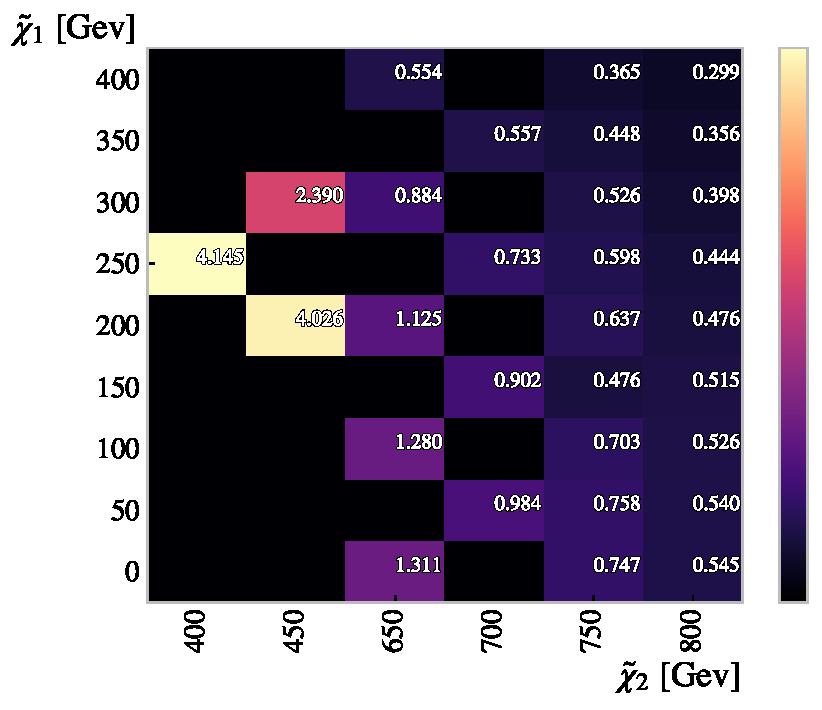
\includegraphics[width=\textwidth]{Figures/MLResults/NN/SUSY/Grid/PNNGridSig.pdf}
    \end{subfigure}
    }
    \caption{A grid displaying the expected significance on the original signal set using the signal region 
    created by the \acs{PNN}.}
    \label{fig:PNNGridSig}
\end{figure}
In this analysis I choose to follow the methodology described in the article by Baldi et al. \cite{PNN}, but other variants of the \ac{PNN} could 
be of interest in future studies. An alternative to the current setup for distributing parameters to the background, is to distribute the parameters evenly. 
In other words, for N different mass combinations, each set of parameters will be randomly distributed to 1/N parts of the background. This would most likely produce a
more balanced result. I considered using an even approach, but found that the current setup was more aligned with the rest of the analysis where a one-one, signal-
background ratio approach has been made\footnote{In section \ref{subsec:TraVal} I discuss how I have chosen to scale the weights such that sum of the weights of 
the background is equal to the sum of the weights of the signal.}. The more interesting alternative would be to assign the background most similar to a given mass 
combination\footnote{By most similar I refer to the background with the largest overlap in the feature space to the signal.}, the same parameters. This would 
focus the training of the \ac{PNN} on the set of events which should be hardest to separate. One approach to determine which events are deemed 'most similar' to a 
combination, is to apply a prior \ac{ML} analysis with a simple \ac{BDT} or dense \ac{NN}. Due to time constraints of this thesis, I decided not to test this 
approach, but would be an interesting area to explore.